\documentclass[twoside,11pt]{homework}

\coursename{COMS 4772 Fall 2015} % DON'T CHANGE THIS

\studentname{Daniel Kronovet}       % YOUR NAME GOES HERE
\studentmail{dbk2123@columbia.edu}   % YOUR UNI GOES HERE
\homeworknumber{2}               % THE HOMEWORK NUMBER GOES HERE
\collaborators{Stephen Ra, Steve Royce}             % THE UNI'S OF STUDENTS YOU DISCUSSED WITH

\begin{document}
\maketitle

\section*{Problem 1}

We set up the EM master equation across variables $X, W, Z$ as follows:

\[
ln p(X,W) =
\int q(Z) ln \frac{p(X, W, Z)}{q(Z)} dZ +
\int q(Z) ln \frac{q(Z)}{p(Z|X,W)} dZ
\]

Given that $X = (x_1, ..., x_n)$ and $Z = (z_1, ..., z_n)$, and are independent, we can write the joint likelihood as follows:

\[
ln \sum_i^n p(x_i,W) =
\sum_i^n \int q(z_i) ln \frac{p(x_i, W, z_i)}{q(z_i)} dz_i +
\sum_i^n \int q(z_i) ln \frac{q(z_i)}{p(z_i|x_i,W)} dz_i
\]

Finally, we expand the joint distribution into the product of distributions across $x_i, W, z_i$:

\[
ln \sum_i^n p(x_i,W) =
\sum_i^n \int q(z_i) ln \frac{p(x_i|W, z_i)p(W)P(z_i)}{q(z_i)} dz_i +
\sum_i^n \int q(z_i) ln \frac{q(z_i)}{p(z_i|x_i,W)} dz_i
\]

Now, for the E-step of the algorithm, we must derive the posterior distribution $p(z_i|x_i, W)$. We begin with:

\[
p(z_i|x_i, W) =
\frac{
p(x_i|W, z_i)p(W)p(z_i)
}{
\int p(x_i|W, z_i)p(W)p(z_i) dz_i
}
\]

As we are not interested in a posterior on $W$, we can treat it as a parameter, and thus cancel it out:

\[
p(z_i|x_i, W) =
\frac{
p(x_i|W, z_i)p(z_i)
}{
\int p(x_i|W, z_i)p(z_i) dz_i
}
\]

Now we are dealing with the posterior over two Gaussians, which is itself Gaussian. We focus on the numerator, with the denominator ultimately providing the normalizing constant.

\[
p(x_i|W, z_i)p(z_i)
\]

\[
(2\pi)^{-d/2}(|\sigma^2 I|)^{-1/2}exp\Braces{-\frac{1}{2}(x_i-Wz_i)^T(\sigma^2I)^{-1}(x_i-Wz_i)}
(2\pi)^{-k/2}(|I|)^{-1/2}exp\Braces{-\frac{1}{2}(z_i)^T(I)^{-1}(z_i)}
\]

\[
(2\pi)^\frac{-d+k}{2}(|\sigma^2 I|)^{-1/2}exp\Braces{-\frac{1}{2}\Brackets{(x_i-Wz_i)^T(\sigma^2I)^{-1}(x_i-Wz_i) + (z_i)^T(z_i)}}
\]

To finish the derivation, we turn to Bishop 2.3, which gives $z_i \sim N(\mu_i^\prime, \Sigma_i^\prime)$:

\[
\Sigma_i^\prime = \Parens{I + \frac{W^TW}{\sigma^2}}, \mu_i^\prime = \Sigma_i^\prime\frac{W^Tx_i}{\sigma^2}
\]

With the posterior in hand, we can return to the EM master equation to complete the E-step by setting $q(z_i) = p(z_i|x_i, W)$, with $W = W_t$, the value of $W$ at the t-th iteration of our algorithm:

\[
ln \sum_i^n p(x_i,W) =
\underbrace{
\sum_i^n \int p(z_i|x_i, W) ln \frac{p(x_i|W, z_i)p(W)p(z_i)}{p(z_i|x_i, W)} dz_i}_{\mathcal{L}(W_t)} +
\underbrace{
\sum_i^n \int p(z_i|x_i, W)ln \frac{p(z_i|x_i, W)}{p(z_i|x_i,W)} dz_i}_{\text{KL-Divergence}}
\]

We now attempt to find $W_{t+1}$ by maximizing $\mathcal{L}(W)$.

\[
\mathcal{L}(W) = \sum_i^n \int p(z_i|x_i, W) ln \frac{p(x_i|W, z_i)p(W)p(z_i)}{p(z_i|x_i, W)} dz_i
\]

\[
= \sum_i^n \int p(z_i|x_i, W) ln p(x_i|W, z_i)p(W)p(z_i) dz_i - 
\int p(z_i|x_i, W) ln p(z_i|x_i, W) dz_i
\]

The left-hand term, the entropy of $q(z_i)$, does not depend on $W$, and can be excluded from the optimization.

\[
\sum_i^n \int p(z_i|x_i, W) ln p(x_i|W, z_i)p(W)p(z_i) dz_i
+ const
\]

\[
= \sum_i^n \bbE_q \Brackets{ln p(x_i|W, z_i)p(W)p(z_i)}
+ const
\]

\[
= \sum_i^n \bbE_q \Brackets{ln p(x_i|W, z_i)} +
\bbE_q \Brackets{lnp(W)} +
\bbE_q \Brackets{lnp(z_i)}
+ const
\]

Again, we can drop the left-most term, which does not vary with $W$ and will disappear once we take the derivative.

\[
= \sum_i^n \bbE_q \Brackets{ln p(x_i|W, z_i)} +
\bbE_q \Brackets{lnp(W)}
+ const
\]

We now expand into the distributions:

\[
= \sum_i^n
\bbE_q \Brackets{-\frac{d}{2}ln(2\pi) - \frac{1}{2}ln(|I\sigma^2|) - \frac{1}{2\sigma^2}||x_i - Wz_i||_2^2} +
\bbE_q \Brackets{\frac{dk}{2}ln\Parens{\frac{\lambda}{2\pi}} - \frac{\lambda}{2}trace(W^TW)}
+ const
\]

We take advantage of the linearity of expectation:

\[
= \sum_i^n
-\frac{d}{2}ln(2\pi) - \frac{1}{2}ln(|I\sigma^2|) - \frac{1}{2\sigma^2}
\bbE_q \Brackets{
||x_i - Wz_i||_2^2
} +
\frac{dk}{2}ln\Parens{\frac{\lambda}{2\pi}} - \frac{\lambda}{2}trace(W^TW)
+ const
\]

And again exclude every term not involving $W$. 

\[
= \sum_i^n
- \frac{1}{2\sigma^2}
\bbE_q \Brackets{
||x_i - Wz_i||_2^2
}
- \frac{\lambda}{2}trace(W^TW)
+ const
\]

We now expand the quadratic term.

\[
= \sum_i^n
- \frac{1}{2\sigma^2}
\bbE_q \Brackets{
||x_i||
- 2x_i^TWz_i
+ ||Wz_i||
}
- \frac{\lambda}{2}trace(W^TW)
+ const
\]

And carry through the expectation.

\[
= \sum_i^n
- \frac{1}{2\sigma^2}
\Parens{||x_i|| - 2x_i^TW
\bbE_q \Brackets{
z_i
} + \bbE_q \Brackets{
||Wz_i||
}
}
- \frac{\lambda}{2}trace(W^TW)
+ const
\]

\[
= \sum_i^n
- \frac{1}{2\sigma^2}
\Parens{||x_i|| - 2x_i^TW\mu_i^\prime
+ \bbE_q \Brackets{
||Wz_i||
}
}
- \frac{\lambda}{2}trace(W^TW)
+ const
\]

\[
= \sum_i^n
- \frac{1}{2\sigma^2}
||x_i||
+ \sum_i^n
\frac{1}{\sigma^2} x_i^TW\mu_i^\prime
- \sum_i^n
\frac{1}{2\sigma^2} \bbE_q \Brackets{||Wz_i||}
- \frac{\lambda}{2}trace(W^TW)
+ const
\]

At last, we take the derivative of $\mathcal{L}(W)$:

\[
\mathcal{L}_{\nabla_W} =
\sum_i^n
\frac{1}{\sigma^2} x_i\mu_i^{\prime T}
- \sum_i^n
\frac{1}{2\sigma^2} \bbE_q \Brackets{2(Wz_i)z_i^T}
- \frac{\lambda}{2}2W
= 0
\]

\[
\sum_i^n
\frac{1}{\sigma^2} x_i\mu_i^{\prime T}
- \sum_i^n
\frac{1}{\sigma^2}W \bbE_q \Brackets{z_iz_i^T}
- \lambda W
= 0
\]

\[
\sum_i^n
\frac{1}{\sigma^2} x_i\mu_i^{\prime T}
- \sum_i^n
\frac{1}{\sigma^2}W (\Sigma_i^\prime + \mu_i^\prime \mu_i^{\prime T})
- \lambda W
= 0
\]

Reorganizing:

\[
\sum_i^n
x_i\mu_i^{\prime T}
=
W \Brackets{\sum_i^n
(\Sigma_i^\prime + \mu_i^\prime \mu_i^{\prime T})
+ \sigma^2 \lambda
}
\]

\[
\Brackets{\sum_i^n 
x_i\mu_i^{\prime T}}
\Brackets{\sum_i^n
(\Sigma_i^\prime + \mu_i^\prime \mu_i^{\prime T})
+ \sigma^2 \lambda
}^{-1}
= W = 
W_{t+1}
\]

Finishing the derivation.

To run the actual algorithm, we first set $q(z_i) = p(z_i | x_i, W_t)$, which allows us to generate $\mathcal{L}_{W_{t}}$.

Then, we take the derivative of this $\mathcal{L}_{W_{t}}$ with respect to $W$ to find the value $W_{t+1}$ which maximizes $\mathcal{L}_{W_{t}(W)}$.

Once we have this new $W_{t+1}$, we can calculate the new $q(z_i) = p(z_i | x_i, W_{t+!})$.
From here, we can repeat the process to derive better and better value of $W$, our model variable of interest.

\section*{Problem 2}

\textbf{Part a}

I did this it was fun.

\textbf{Part b}

Log likelihood at T=100

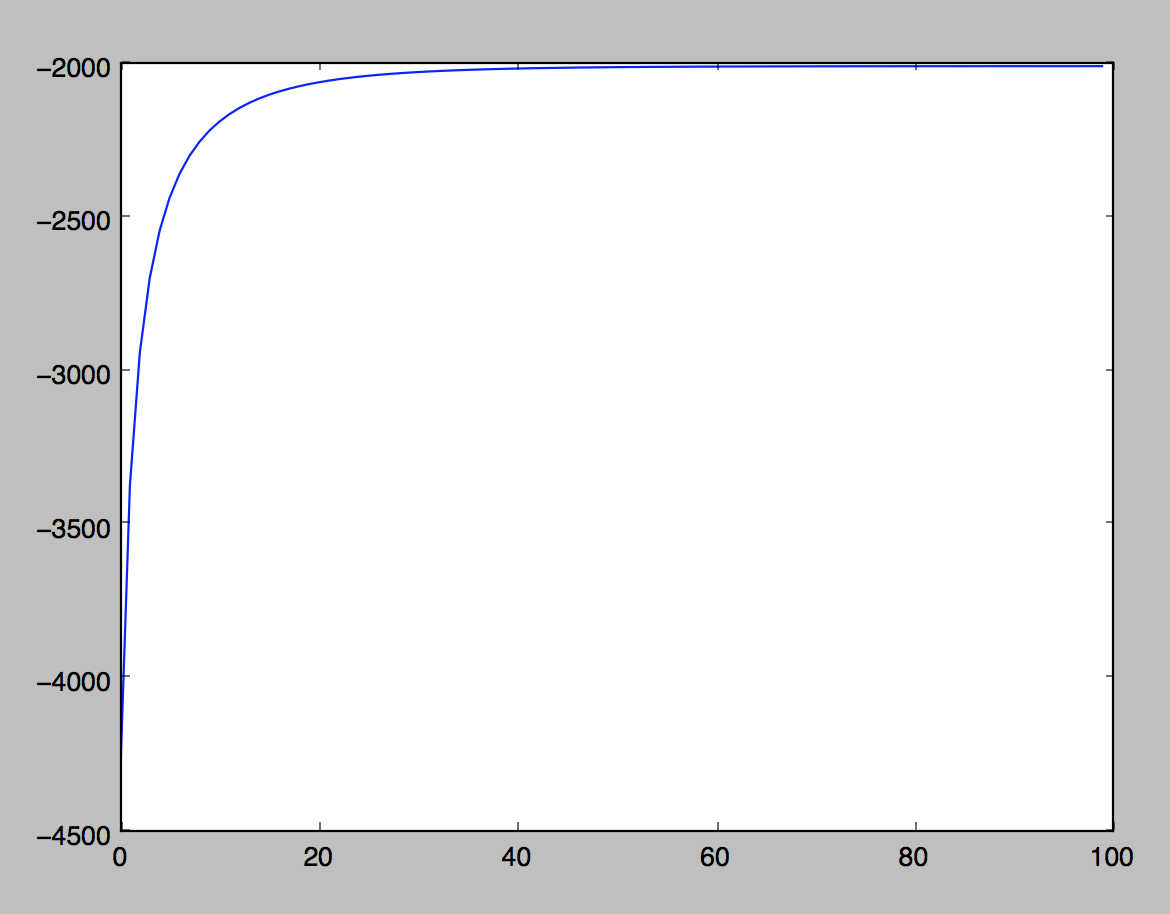
\includegraphics[scale=.5]{images/loglikelihood.png}

\textbf{Part c}

\begin{center}
  \begin{tabular}{c||c|c|c|c}
    & 0
    & 1 \\
    \hline
    \hline
    $0$
    & 931
    & 51
    \\
    \hline
    $1$
    & 77
    & 932
  \end{tabular}
\end{center}

\[
Accuracy = 0.935710698142
\]

\textbf{Part d: Misclassified Images}

Image 156, $\sim Bern(0.836626)$

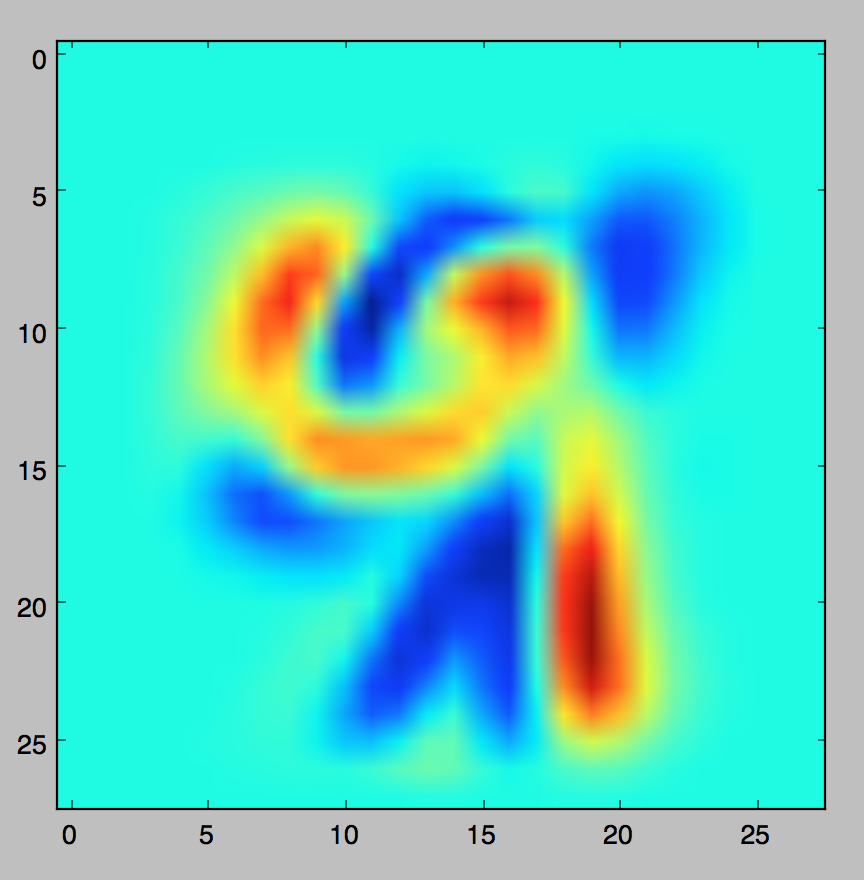
\includegraphics[scale=.5]{images/156.png}

Image 564, $\sim Bern(0.584582)$

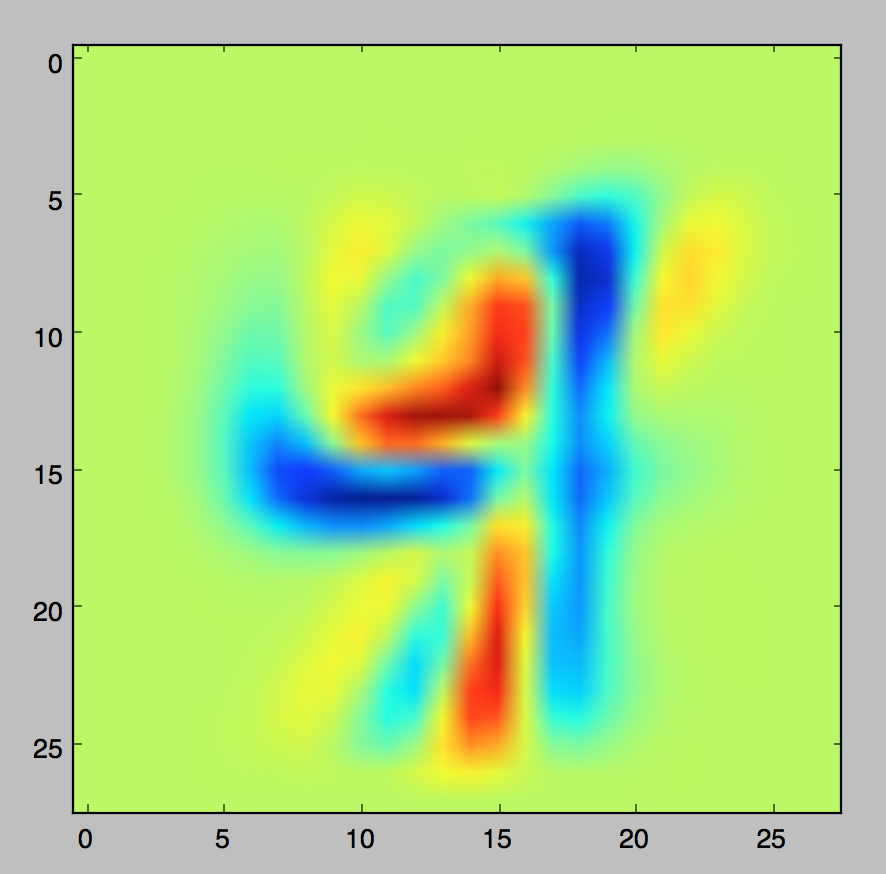
\includegraphics[scale=.5]{images/564.png}

Image 1658, $\sim Bern(0.47498)$

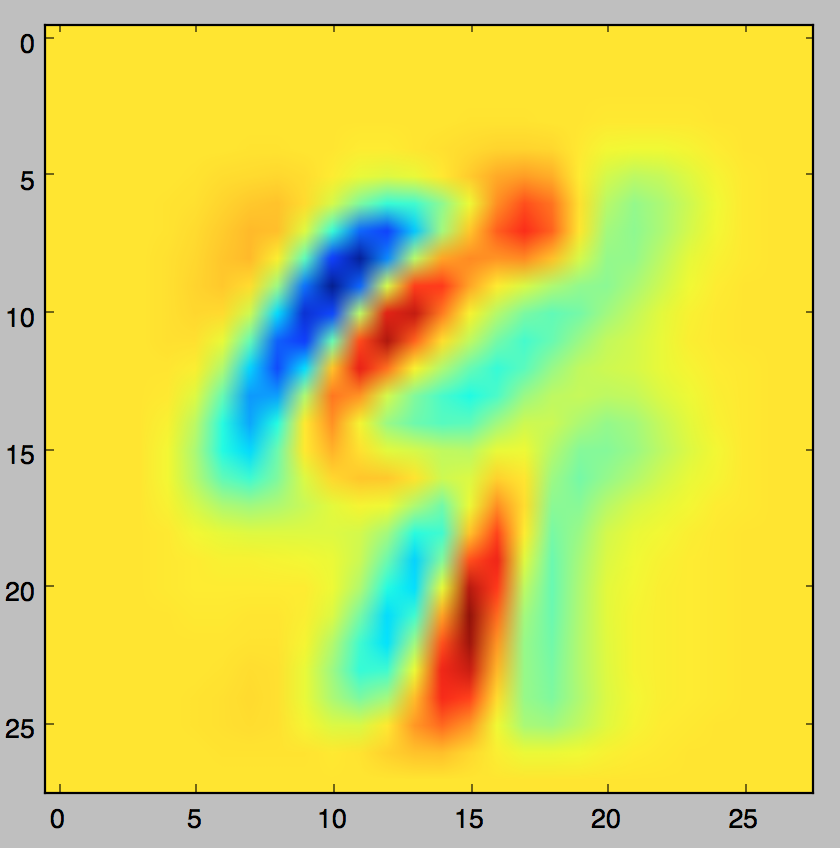
\includegraphics[scale=.5]{images/1658.png}

\textbf{Part e: Ambiguous Predictions}

Image 210, $\sim Bern(0.502074)$

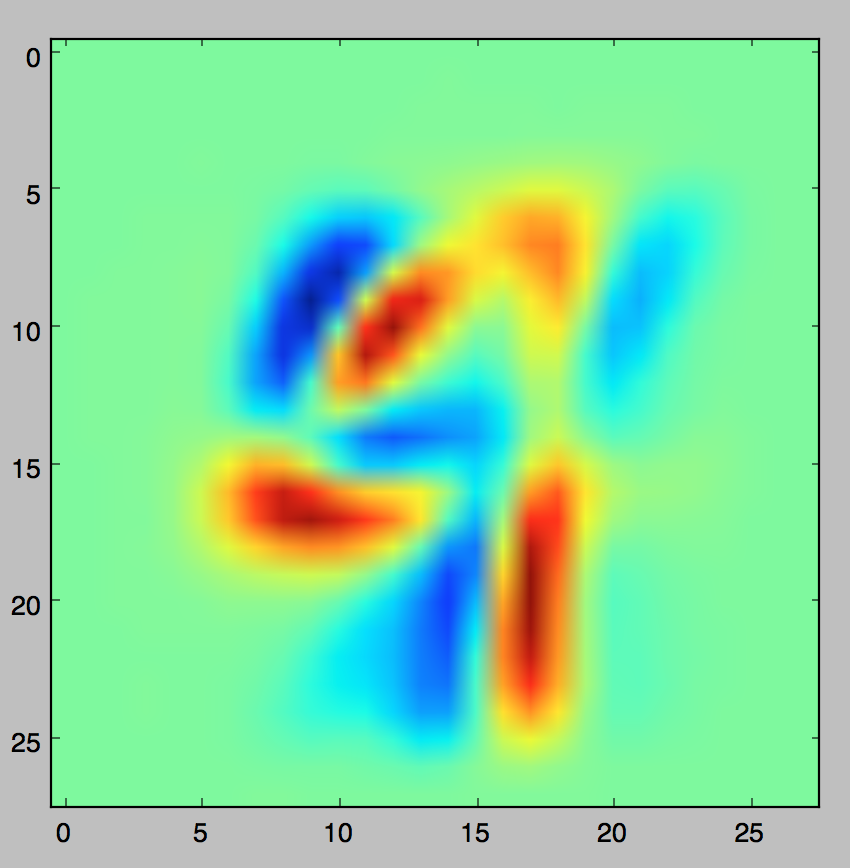
\includegraphics[scale=.5]{images/210.png}

Image 340, $\sim Bern(0.505406)$

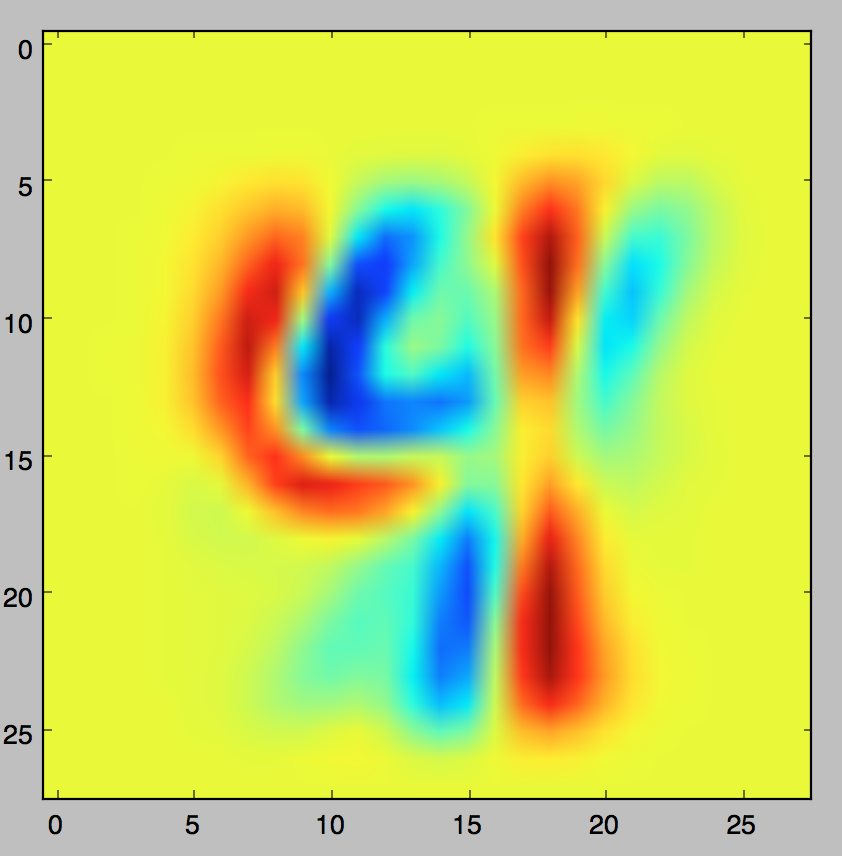
\includegraphics[scale=.5]{images/340.png}

Image 1990, $\sim Bern(0.501256)$

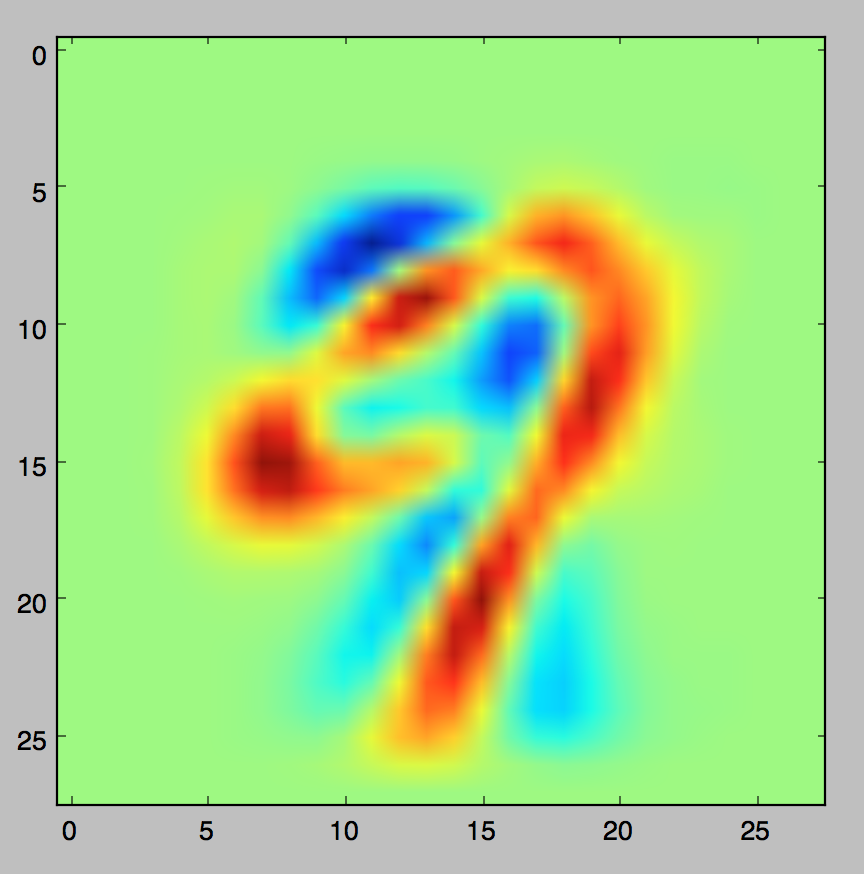
\includegraphics[scale=.5]{images/1990.png}

\textbf{Part e: Changes to w over time}

T=1

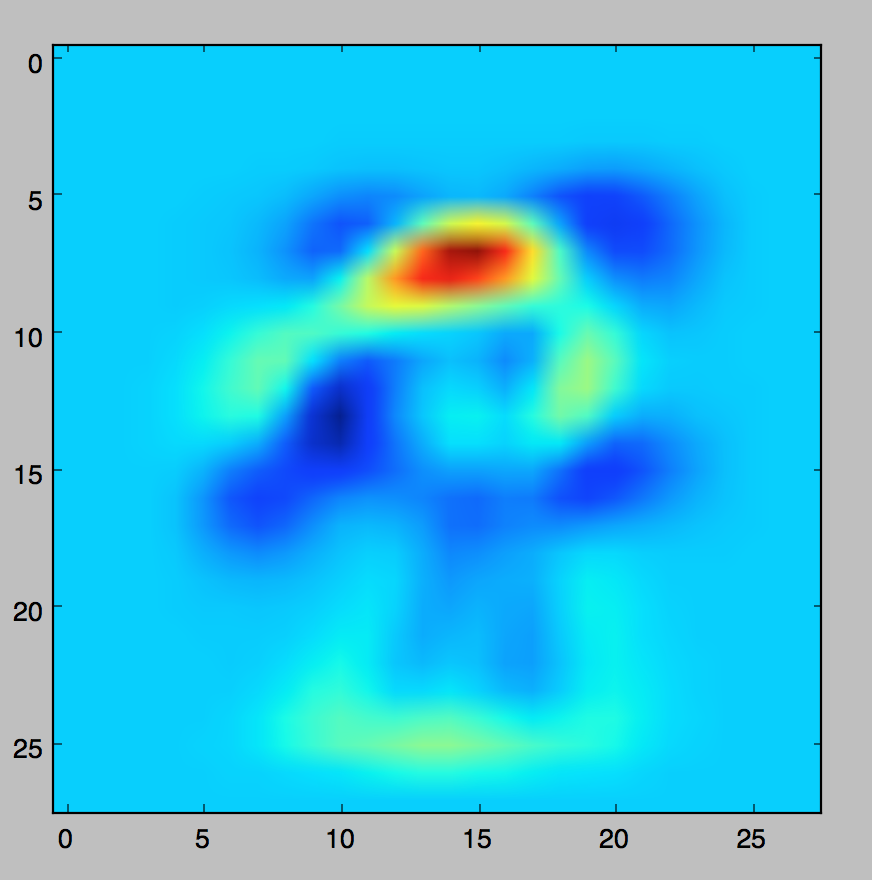
\includegraphics[scale=.5]{images/w1.png}

T=5

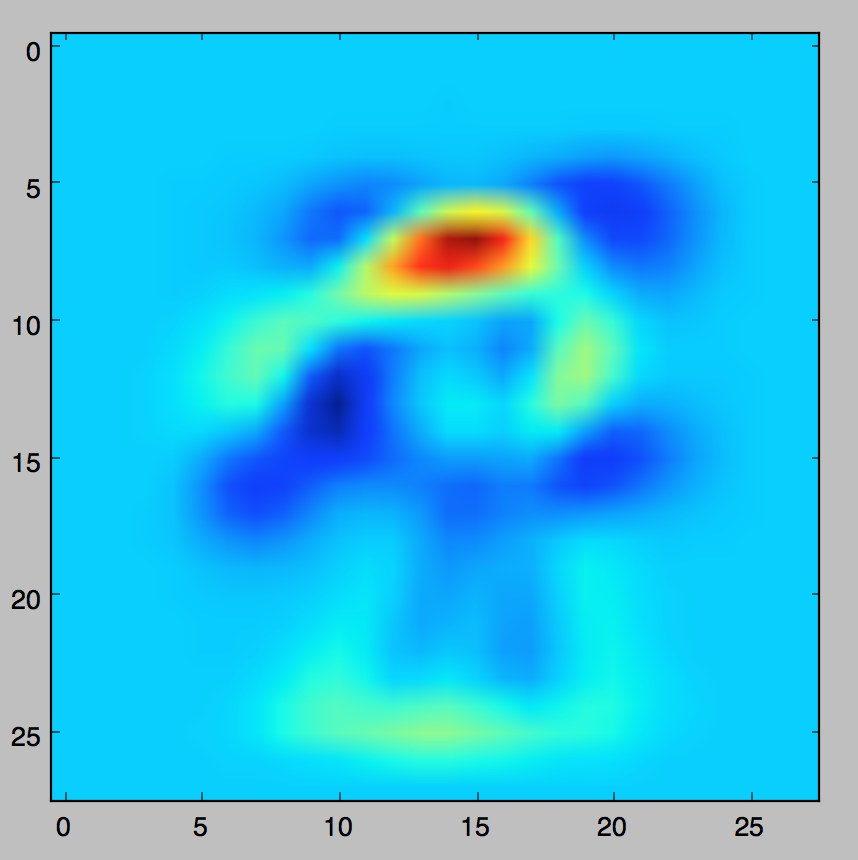
\includegraphics[scale=.5]{images/w5.png}

T=10

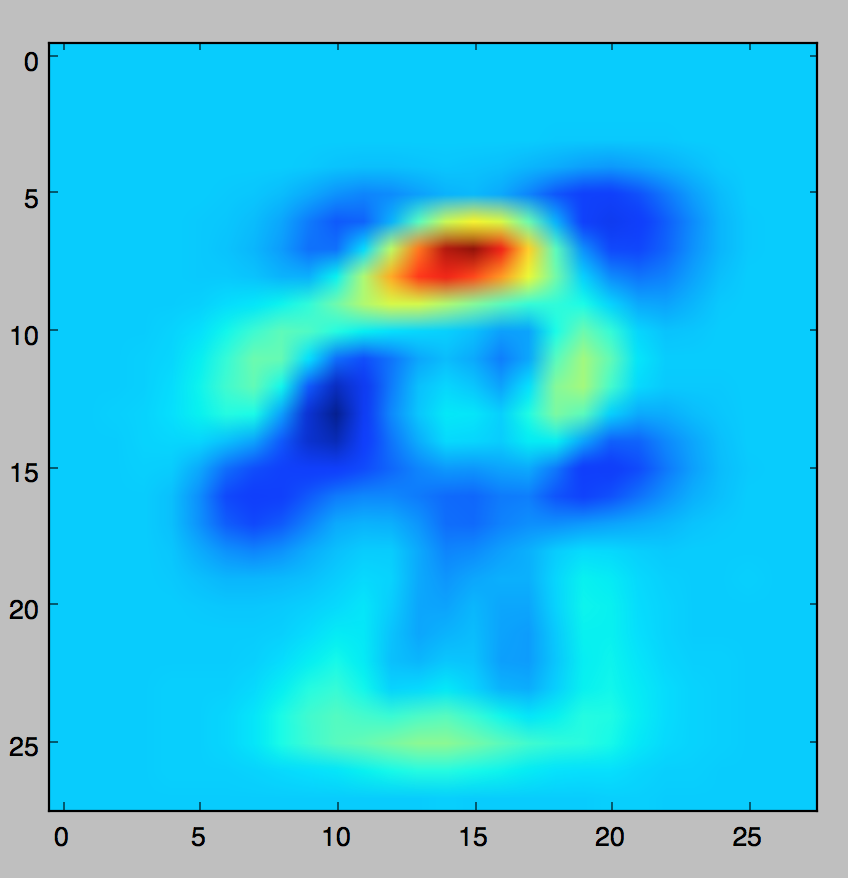
\includegraphics[scale=.5]{images/w10.png}

T=25

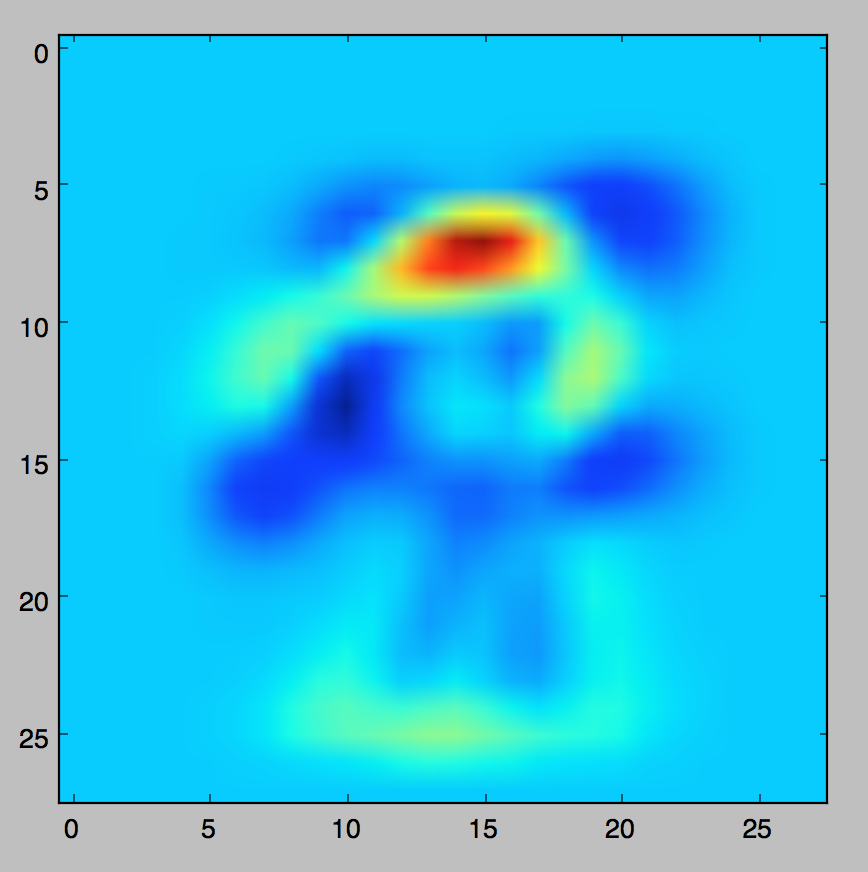
\includegraphics[scale=.5]{images/w25.png}

T=50

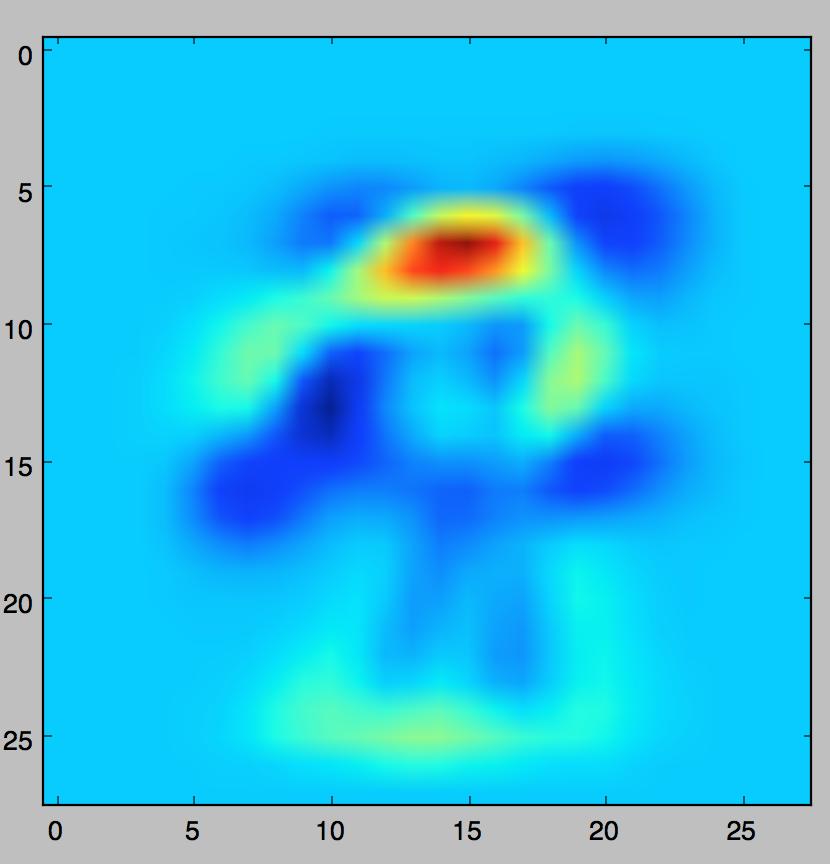
\includegraphics[scale=.5]{images/w50.png}

T=100

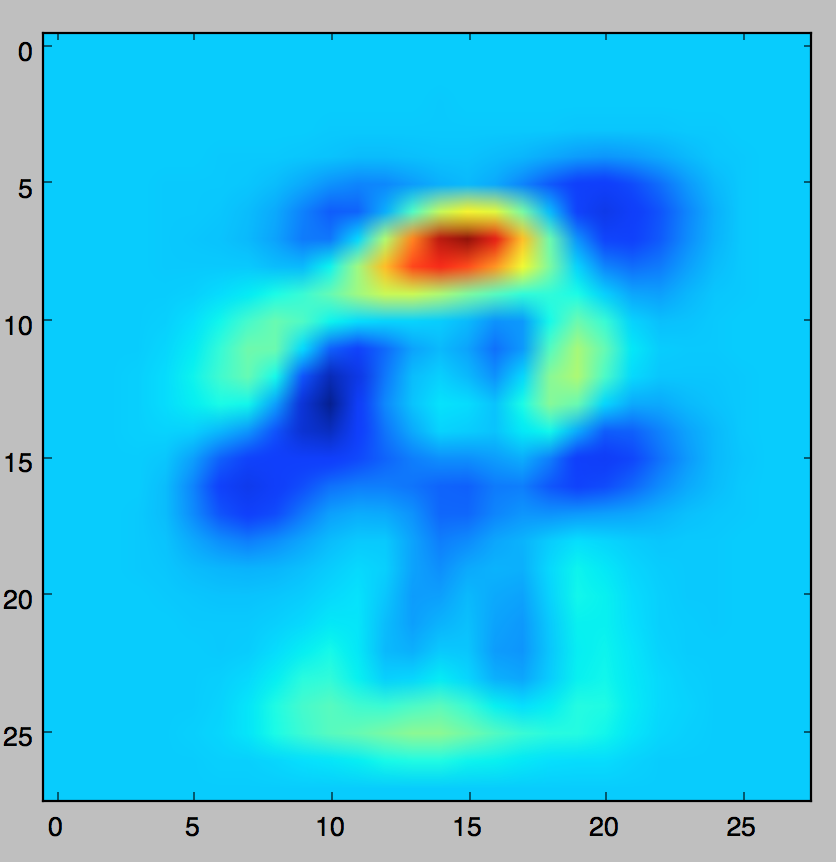
\includegraphics[scale=.5]{images/w100.png}

I noticed relatively little change in the rendered w.
There were small changes in the distribution of heat across the image,
which I interpret as the algorithm learning more precisely which components of a handwritten image are the most powerful discriminators.

\end{document} 
